%----------------------------------------------------------------------------
\chapter{Own work}\label{ch:own-work}
%----------------------------------------------------------------------------

In this chapter, I will describe my work, from the specification of the task through the testing process to the results. The structuring of the experiments will mostly follow a chronological timeline, with the most basic questions answered first.

\section{Defining the objective}\label{sec:defining-the-objective}

The first problem I encountered during my work was that there is no clear definition of what a good embedding is. No simple metric exists that accurately and fully captures the nuances of embedding a latent chemical space in lower dimension. This is not surprising, since the very existence of so many different dimension algorithms comes from the fact that there is no consensus on that a good dimension reduction algorithm does. As such, I needed to define my own metrics for ranking each embedding. For this, I turned to the underlying goal of embedding these molecules.

The main objective of my thesis is exploring the capability of the previously described dimension reduction algorithms in novel drug discovery. Some assumptions must be made for formalizing the requirements. The first such assumption is that molecules that have similar a structure also have similar chemical properties. While this statement is not true for all chemical descriptors, it holds for most non-categorical metrics, such as number of rings in the molecule, or the topological polar surface area (TPSA~\cite{bib:tpsa}). This intuition implies that molecules with similar structure have similar binding properties to certain proteins too, which is the most vital metric for novel drug research. Drug molecules act by binding to proteins, forming complexes that induce physiological changes in the body. The efficacy of binding depends on the chemical properties of the target protein (mainly its three-dimensional shape) and the chemical properties of the drug molecule.

From this, it logically follows that a chemical space that is ordered over the chemical structure of molecules allows the targeted search of potential drug candidates. Unfortunately, chemical structure can not be quantized in such a way as to be able to order them. Instead, I decided that what I needed was a space that \textit{smooth} over chemical structure. In essence, this means that points close to each other have similar chemical structure. This is the exact property that is needed for targeted search. Importantly, this does not imply that points far away from each other have significantly different structure. Optimizing for embedding all similar molecules closely is a difficult task, and I can not be sure that points in the original 64-dimensional dataset even satisfies this condition. An algorithm that places all similarly structured molecules close together is advantageous, but for my purposes, not needed.

In summary, a good embedding is one that is locally smooth over chemical structure. This can most easily be determined by looking at chemical descriptors of molecules, and assessing their local smoothness in the output space.

The choice of descriptors matters greatly in this question. The original model was trained on millions of molecules, and some of their chemical properties. The properties used by the VAE's property predictor was part of the database, which means that the 64-dimensional latent space should in theory be relatively smooth over those metrics. Because of this, the inclusion of other chemical descriptors are needed for a proper examination of data. With mostly smooth transitions on a large number of descriptors, one can be certain that the chemical structure itself changes smoothly.


\begin{itemize}
	\item t-SNE parameter sweep
	\item UMAP sweep
	\item TriMAP sweep
	\item PaCMAP sweep?
	\item LERP - coxib
	\item LERP - random
\end{itemize}

\section{Initial testing}\label{sec:initial-testing}

After defining the objective, the first thing that I did was running each algorithm with default parametrization to see baseline results. This served two purposes. Firstly, by generating baseline embeddings, the effect of different parametrization could be more accurately assessed. Secondly, I recorded the runtime of each algorithm, so their performance could be compared from a different angle.

After running each algorithm once, I noticed that the t-SNE clustering was somewhat strange (as can be seen on figure (\ref{fig:default_run})). The result of this run did not make much sense. It was completely different from what I expected. I had prior experience using t-SNE, albeit another implementation. After rerunning the algorithm, I found a similar result, which led me to believe that the implementation had some bug. Indeed, when I ran t-SNE again in verbose mode, I found that instead of the 2000 iterations specified, it only ran for about 150, which was not enough to form proper clusters. I tried switching to openTSNE, the implementation I used heavily during my project laboratory, however, the sheer size of the dataset made it unusable as the system did not have enough memory to accommodate its needs.

After some consideration, I turned to tsnecuda, another familiar implementation that ran on the GPU (and as such, used its own memory instead of the RAM of the system). I initially chose openTSNE for two reasons: firstly, it was more usable that tsnecuda, as it was far more parametrizable, allowing for custom callback functions and deterministic runs. Secondly, all other algorithm ran on the CPU, making performance comparisons more fair with openTSNE. Since openTSNE could not even complete one run, I was forced to use tsnecuda. This switch however highlighted something very interesting.

In the field of deep learning, GPU's are widely used as they are capable of running thousands of operations in parallel, leading to faster training of models. All graph-based clustering algorithms work very similarly to a neural network, in that they exclusively work with matrices and are highly parallelizable. This means that using GPU resources can significantly speed up the clustering of any given dataset. As can be seen on table (\ref{tab:runtime}), while the sklearn t-SNE implementation took almost exactly 25 hours to run for 150 iterations (plus constructing the higher dimensional probability distribution), tsnecuda did not even take six minutes to perform 5000 iterations (in fact, in the first run, I set it to only 2000 iterations, which ran for 102 seconds, an incredible 883 times faster).

\begin{table}[htb]
	\begin{center}
		\begin{tabular}{|l|r|}
			\hline
			Algorithm (iterations) & runtime \\
			\hline
			PCA & 19.45 s \\
			\hline
			t-SNE (sklearn, 150) & 90 042 s \\
			\hline
			t-SNE (tsnecuda, 5000) & 344.29 s \\
			\hline
			UMAP (1000 epochs) & 5 866.55 s \\
			\hline
			TriMAP (2000) & 26 756.64 s \\
			\hline
			PaCMAP (2000) & 65 283.52 s \\
			\hline
		\end{tabular}
	\end{center}
	\caption{Runtimes of each algorithm tested on the entire dataset (without duplicates, ~1.6 million molecules) given in seconds. The number of iterations and epochs are indicated where applicable. PCA, the only non-iterative method is the fastest, while the others take significantly more time. The power of GPU usage is clearly demonstrated by the two t-SNE implementations.}
	\label{tab:runtime}
\end{table}

Comparison of each algorithm based on the runtimes in table (\ref{tab:runtime}) should only be done in context. PCA is the fastest method of the bunch, this is because it is the only non-iterative algorithm. After that, the GPU implementation of t-SNE is the fastest, but this can not be credited to the algorithm, but the implementation instead. In fact, the slowest running algorithm is also a t-SNE implementation, which ran on the CPU. As for the other graph-based algorithms, they are not equal either. UMAP has multithreaded capabilities, while TriMAP and PaCMAP do not.

In summary, these runtime metrics are not intrinsic properties of the algorithms. They merely describe the performance of the current implementations. In time, more libraries will be available for every algorithm and these numbers will change. t-SNE and UMAP both have GPU implementations which vastly outperform their CPU implementations, and even other algorithms that are supposed to be faster than them. In an engineering application, it is important to consider technical parameters, it should be noted that these parameters change as opposed to each algorithm's performance in terms of the quality of the embedding.

\section{Result of first runs}\label{sec:result-of-first-runs}

I have briefly touched on the importance of chemical descriptors in the inference of structure in section (\ref{sec:defining-the-objective}). Since the original model was trained with a property predictor, it is to be expected that the latent space is smooth over those descriptors. This can be seen on figure (\ref{fig:default_run}) with the quantitative estimate of drug-likeness (qed~\cite{bib:qed}). Additional metrics were needed to properly be able to induce chemical structure. This is needed because while structural similarity between molecules can easily be captured by one number, the structure of individual molecules is typically described by fingerprint vectors. These would form a vector space that is not easy to interpret.

\begin{figure}[!ht]
	\centering
	\includegraphics[width=0.49\columnwidth, keepaspectratio]{figures/PCA_default}
	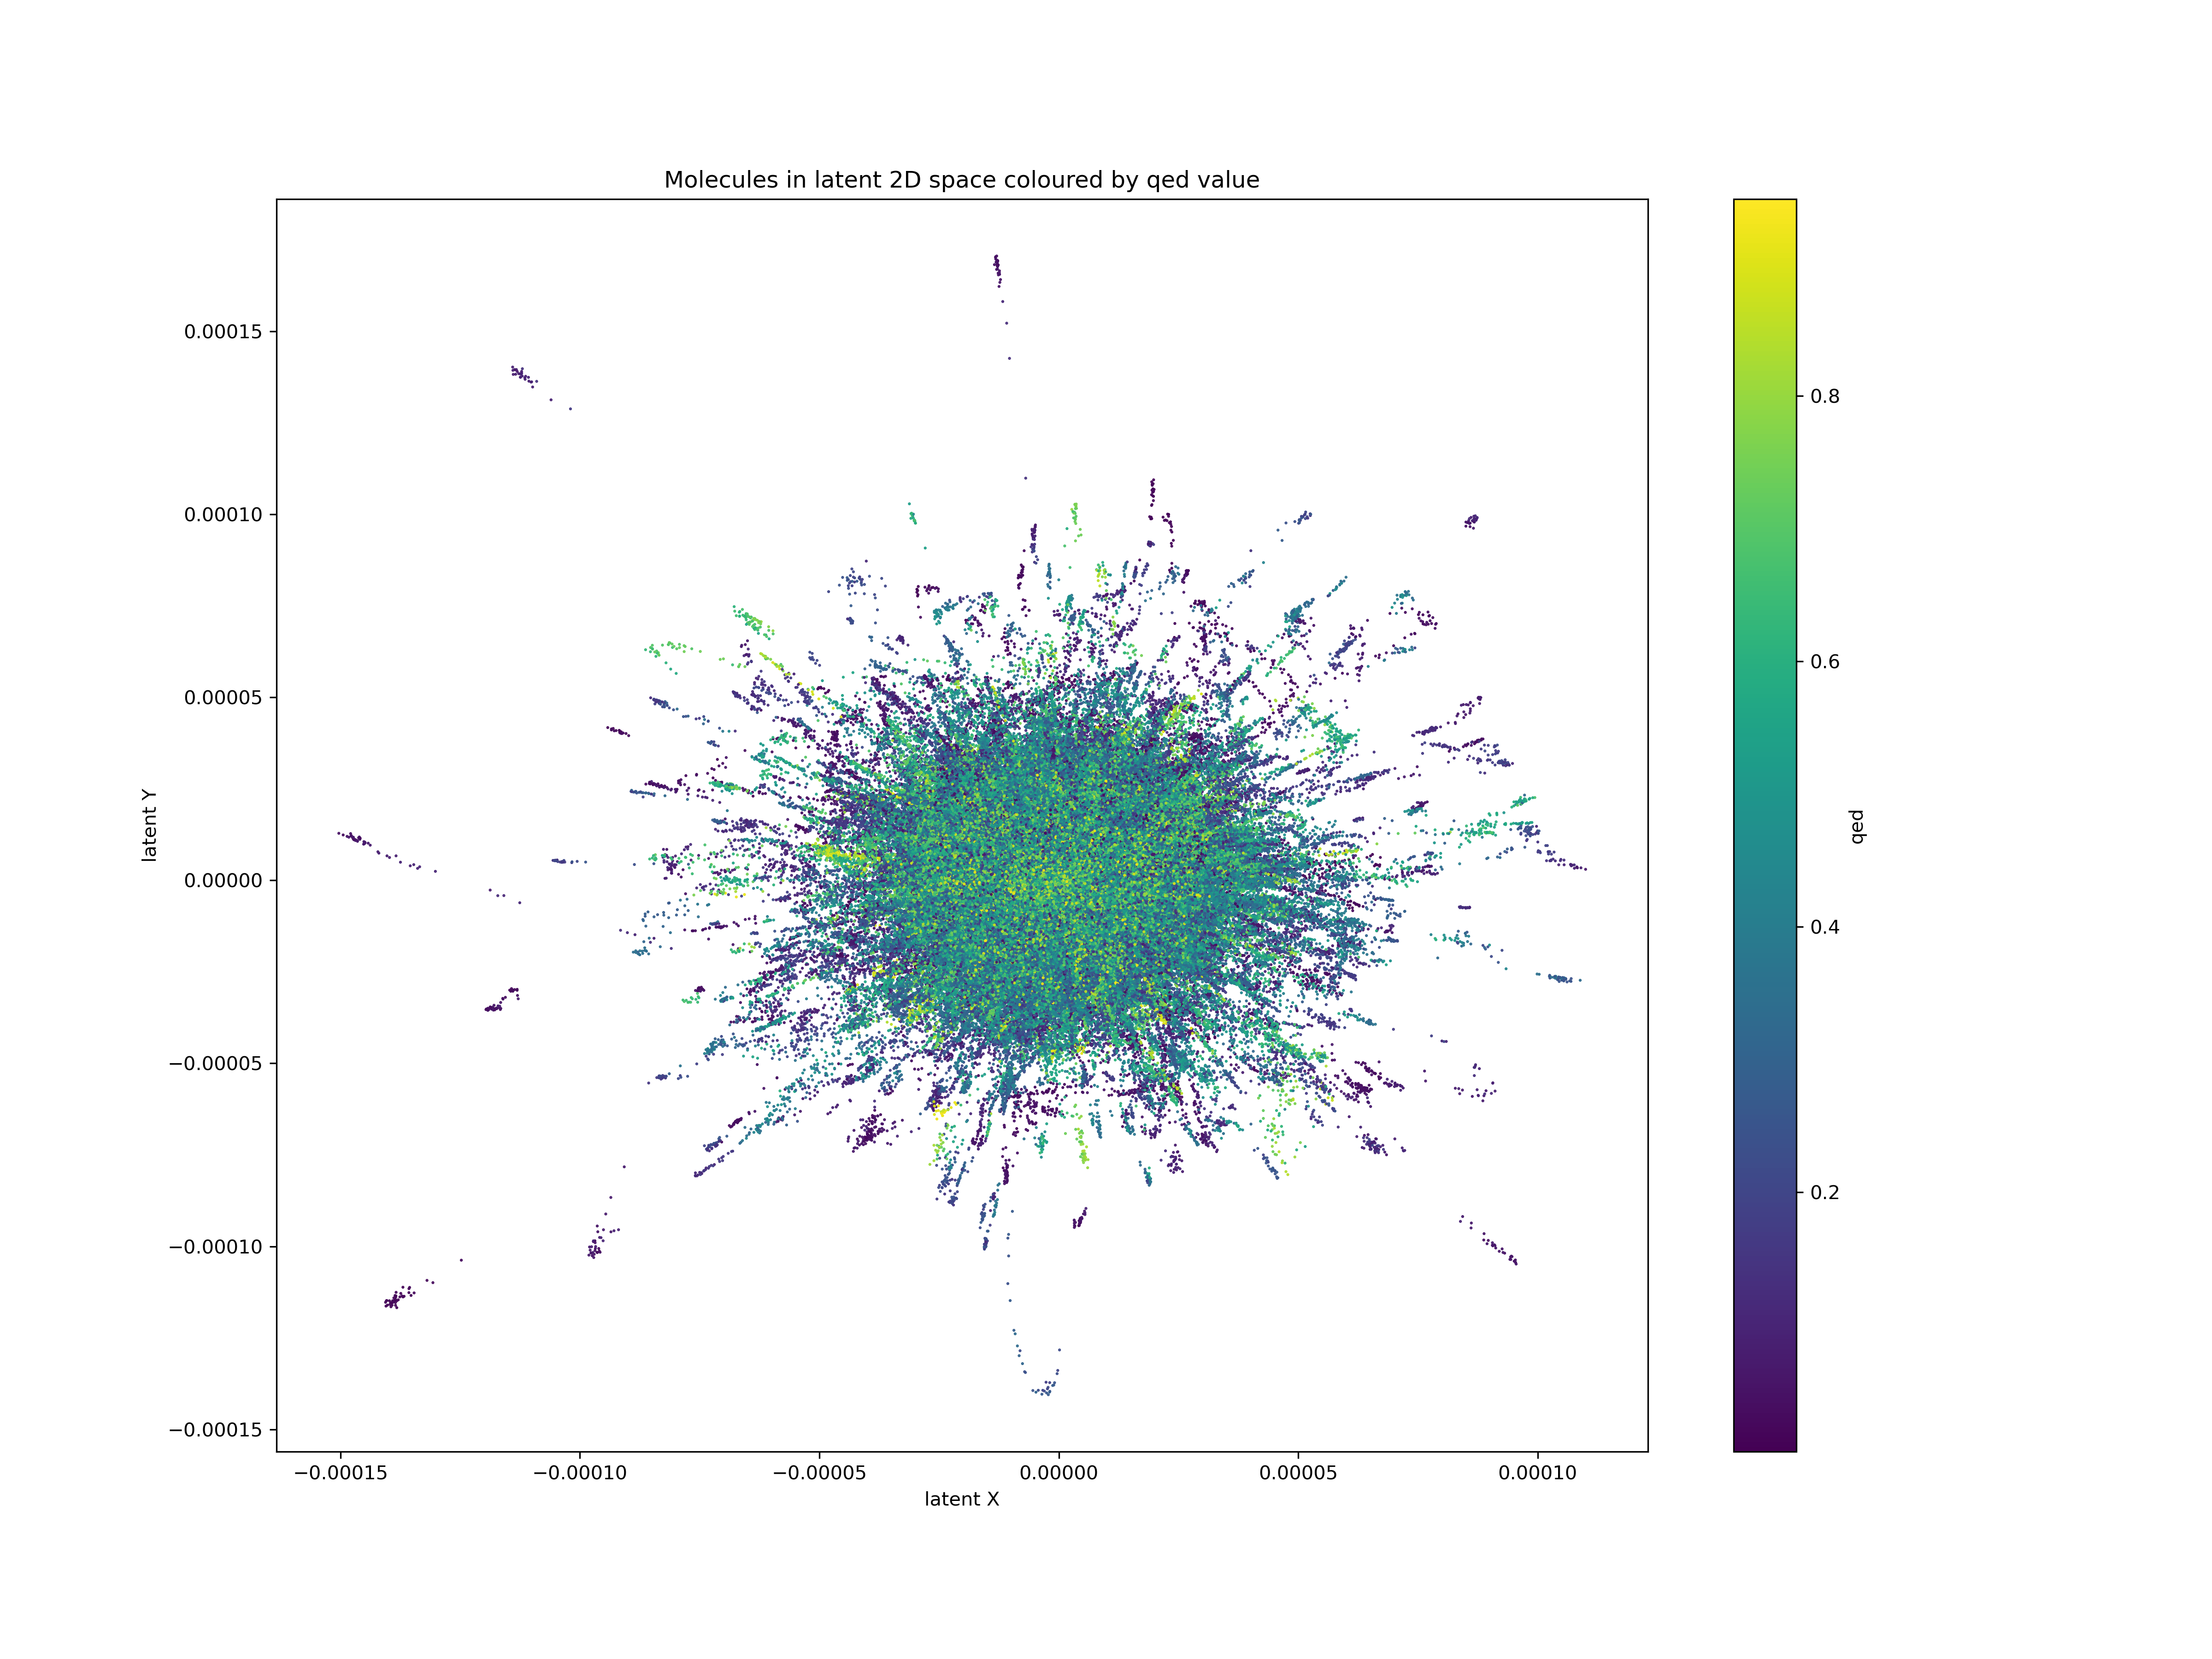
\includegraphics[width=0.49\columnwidth, keepaspectratio]{figures/t-SNE_default}
	\includegraphics[width=0.49\columnwidth, keepaspectratio]{figures/t-SNE2_default}
	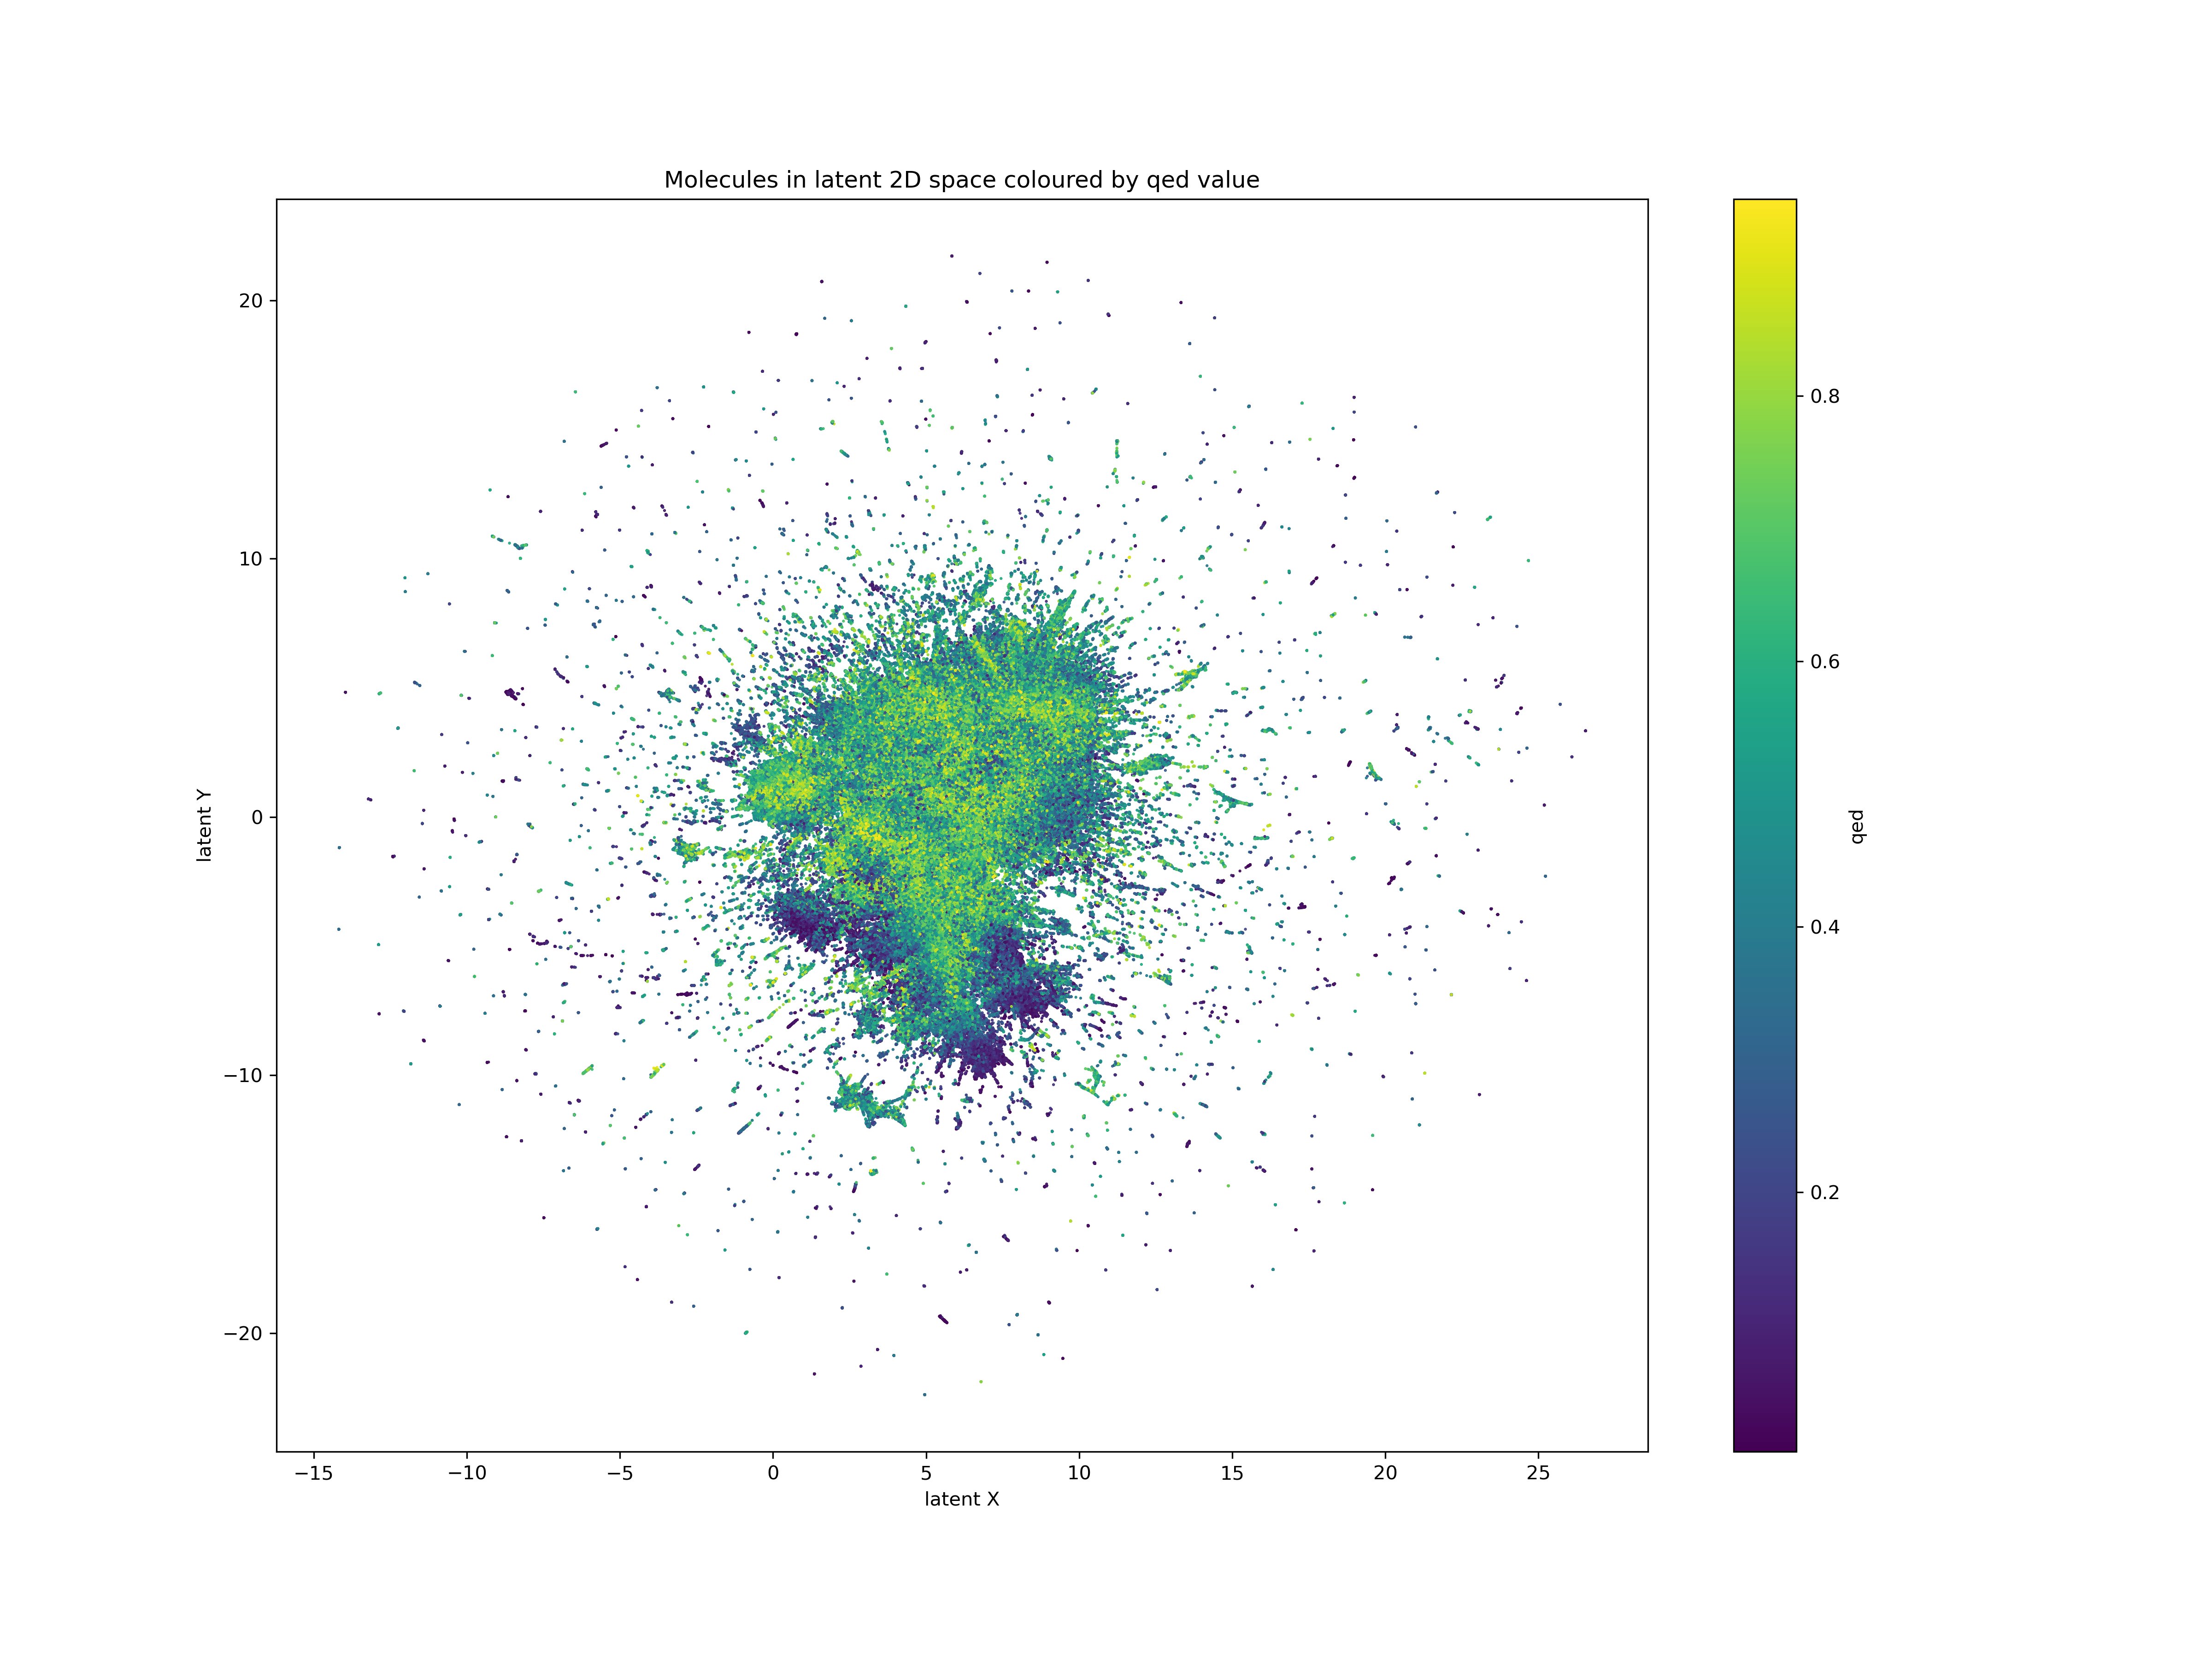
\includegraphics[width=0.49\columnwidth, keepaspectratio]{figures/UMAP_default}
	\includegraphics[width=0.49\columnwidth, keepaspectratio]{figures/TriMAP_default}
	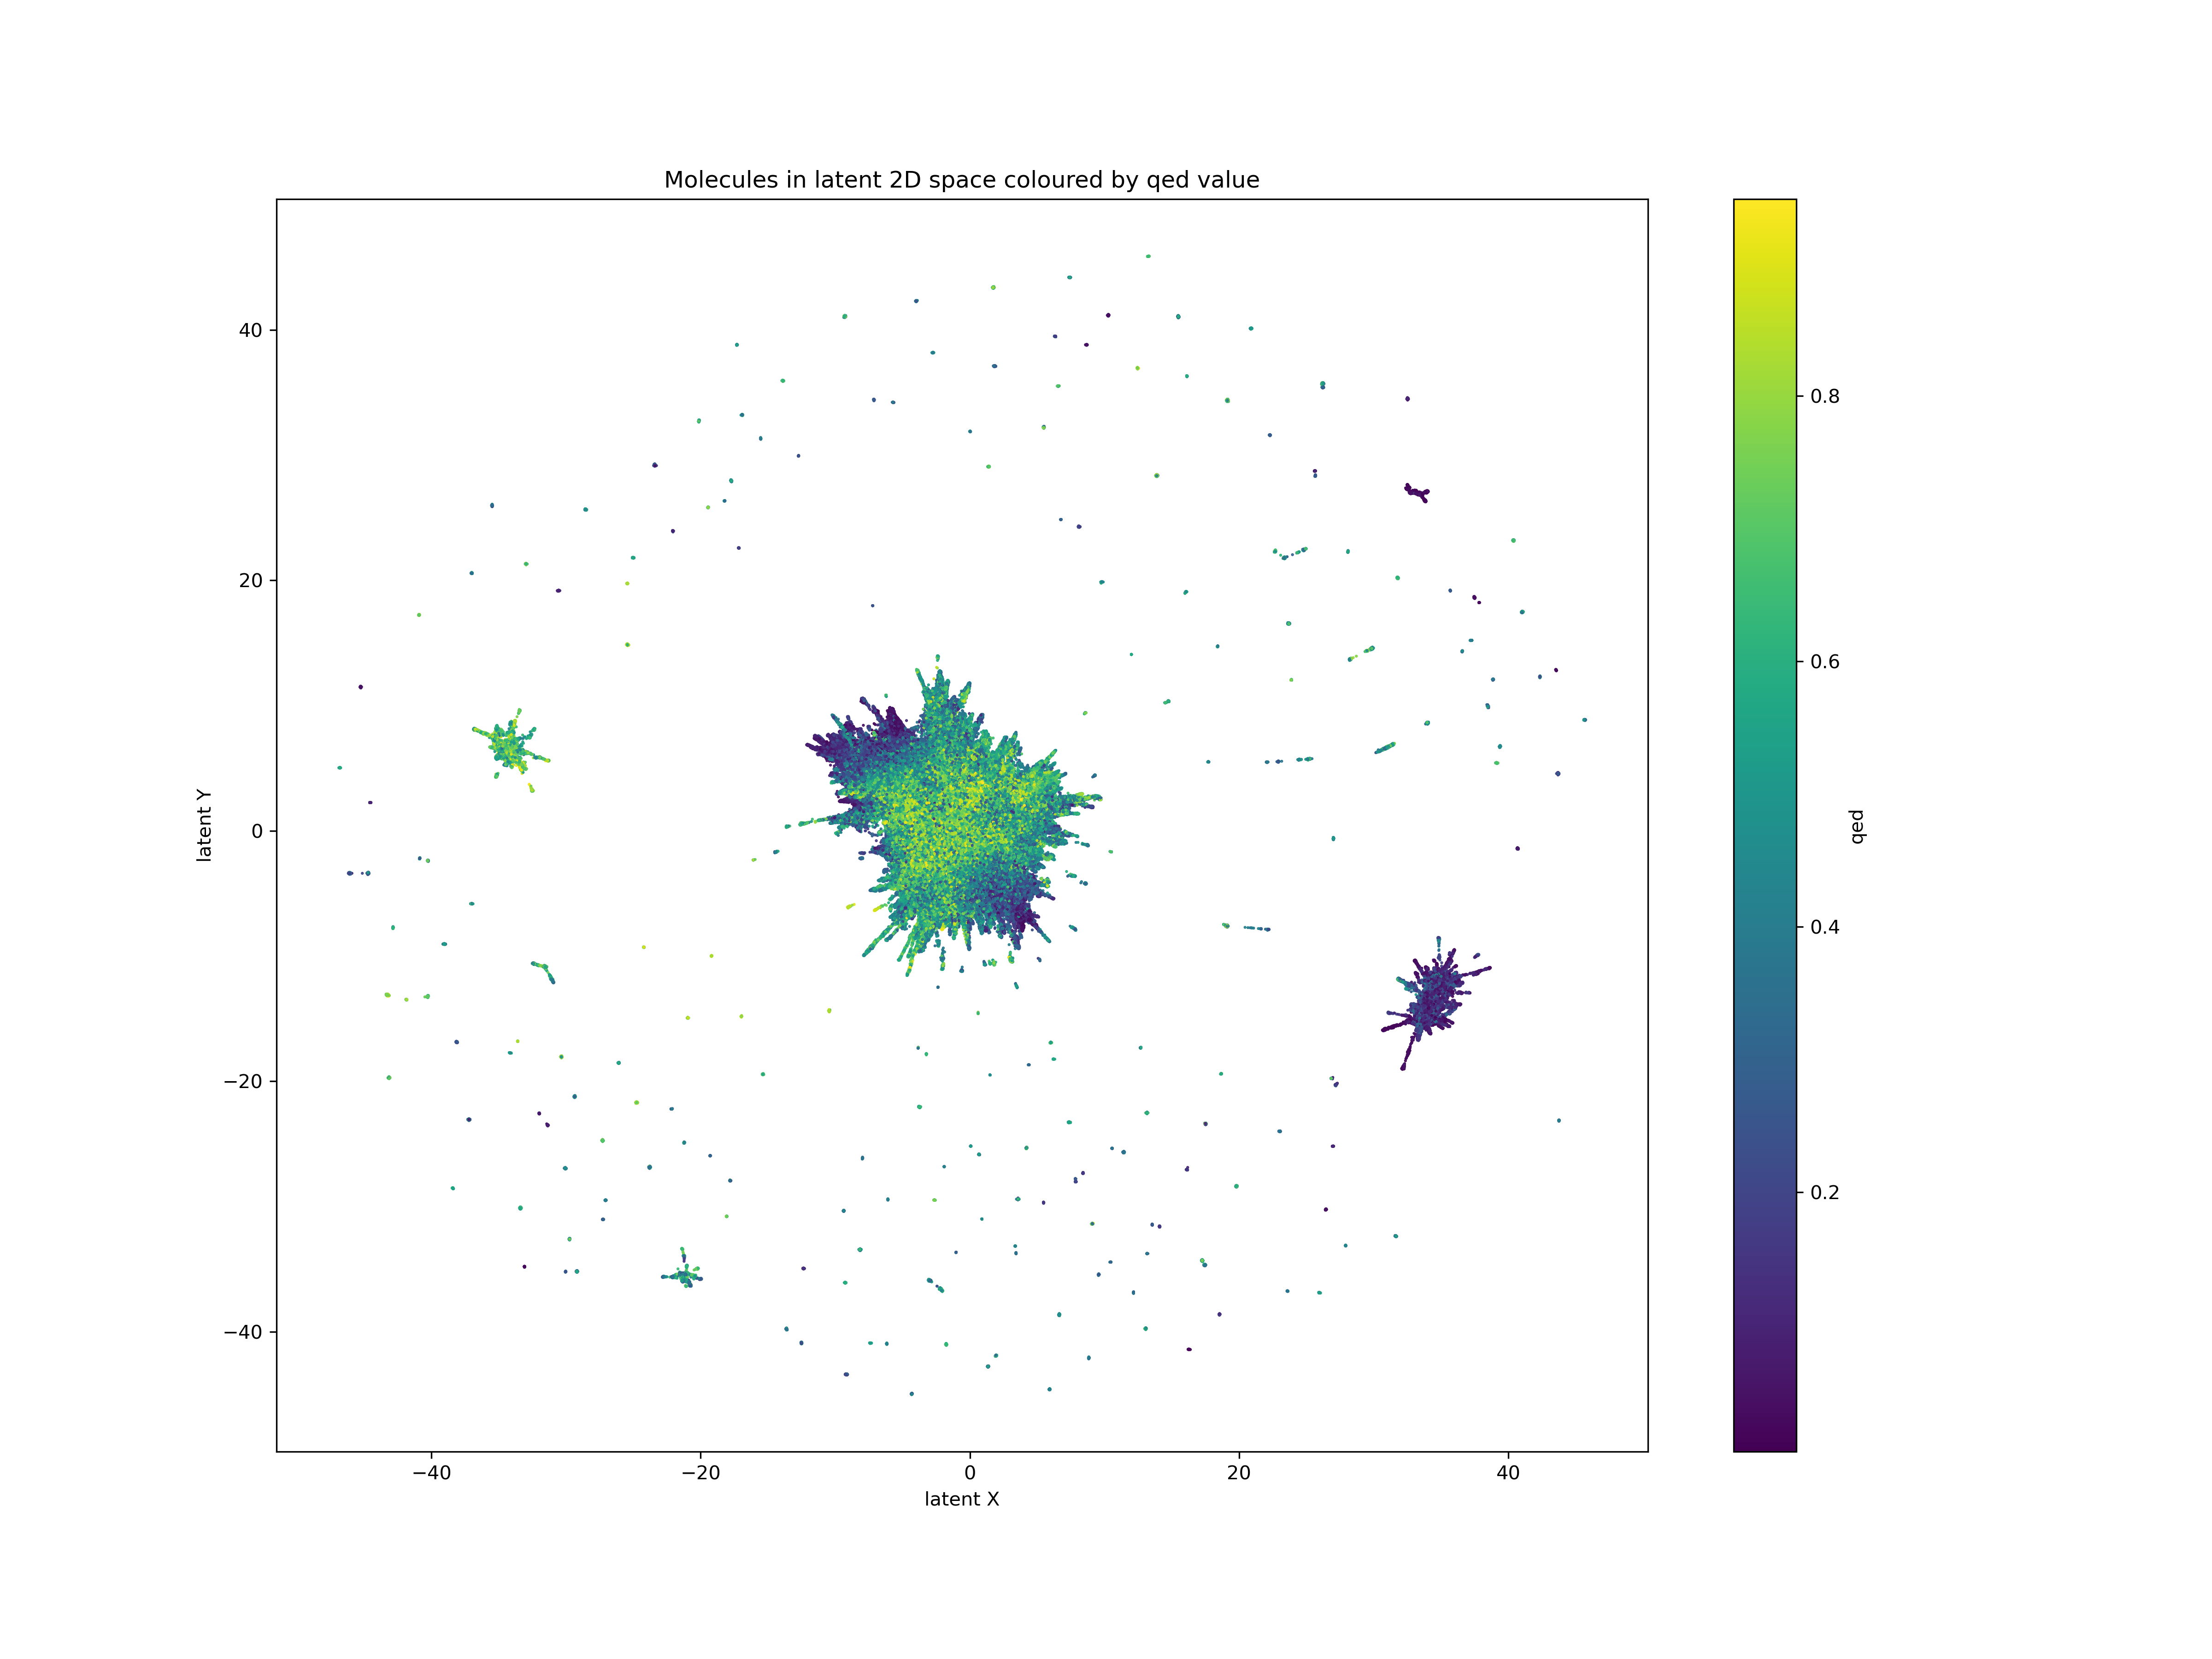
\includegraphics[width=0.49\columnwidth, keepaspectratio]{figures/PaCMAP_default}
	\caption{Results of PCA, t-SNE (sklearn and tsnecuda), UMAP, TriMAP and PaCMAP algorithms on the dataset with default parameters, coloured by the quantitative estimate of drug-likeness of each data point. It can be clearly seen that each algorithm places points very differently.}
	\label{fig:default_run}
\end{figure}

The choice of descriptors matter because different metrics relate differently to chemical structure. For example, the melting point of a substance is affected mostly by the secondary bonds it can form. Consider \textit{ethane} and \textit{ethanol}. These two molecules are structurally very similar, only differing by one oxygen atom. This however changes the strongest secondary bond that can form between individual molecules. While solid ethane is bound together only by \textit{van der Waals forces}~\cite{bib:vanderwaals}, solid ethanol is held together by \textit{hydrogen bonds}~\cite{bib:hbond}, many times stronger. As such, while the melting point of ethane is $-182.8~^\circ$C, ethanol melts at $-114.14~^\circ$C. The difference is even more dramatic for boiling points, $-88.5~^\circ$C and $+78.23~^\circ$C for ethane and ethanol respectively.

The ideal descriptors are those that do not change very much as the structure of molecules changes a little. In the end, I chose the following metrics: Quantitative estimate of drug-likeness, Ring count, number of hydrogen donors, number of hydrogen acceptors, topological polar surface area~\cite{bib:tpsa} and number of rotatable bonds.

It should be noted that some of these descriptors do jump slightly from molecule to molecule, however, this change is not too great to cause problems in interpreting data.

\todo{értékítélet}

\section{Optimizing the parameters}\label{sec:optimizing-the-parameters}



\section{Linear interpolation test}\label{sec:linear-interpolation-test}

